%%%%%%%%%%%%%%%%%%%%%%%%%%%%%%%%%%%%%%%%%%%%%%%%%%%%%%%%%%%%%%%%%%%%%%
%     File: ExtendedAbstract_backg.tex                               %
%     Tex Master: ExtendedAbstract.tex                               %
%                                                                    %
%     Author: Andre Calado Marta                                     %
%     Last modified : 27 Dez 2011                                    %
%%%%%%%%%%%%%%%%%%%%%%%%%%%%%%%%%%%%%%%%%%%%%%%%%%%%%%%%%%%%%%%%%%%%%%
% A Theory section should extend, not repeat, the background to the
% article already dealt with in the Introduction and lay the
% foundation for further work.
%%%%%%%%%%%%%%%%%%%%%%%%%%%%%%%%%%%%%%%%%%%%%%%%%%%%%%%%%%%%%%%%%%%%%%

\section{Flight Dynamics}
\label{sec:backg}

The work made in this article was built on top of the work done by \cite{hector} on 4D trajectory tracking. The model used in this work is a six degree of freedom transport aircraft that will be described in this section. 

\subsection{Frames of Reference}

The first step before describing the dynamics of a commercial aircraft will be to define the frames of reference used to do so. The first frame of reference, on which 4D trajectories are described, corresponds to the WGS84 frame of reference. A second frame of reference corresponding to the aircraft body frame will be used to provide its fast rotational dynamics. Lastly all aerodynamic forces will be applied in the axial directions of the wind frame. This frame is aligned with the wind speed vector relative to the airplane, given by both the angle of attack $\alpha$ and the sideslip angle $\beta$. For these last two frames of reference, a rotation matrix can be defined from wind frame to body frame by


\begin{equation}
R_{BW}=
\begin{bmatrix}
c_\alpha c_\beta & -c_\alpha s_\beta & -s_\alpha \\
s_\beta & c_\beta & 0 \\
s_\alpha c_\beta & -s_\alpha s_\beta & c_\alpha
\end{bmatrix}
\label{eq:wind2body}
\end{equation}

To describe the attitude of the plane Euler, roll, pitch and yaw angles, will also be used, namely $\phi\{-\pi,\pi\}$; $\theta \{-\dfrac{\pi}{2},\dfrac{\pi}{2}\}$; $\psi \{-\pi,\pi\}$. From these angles the rotation matrix from the body to the earth frame is given by

\begin{equation}
R_{EB}=
\begin{bmatrix}
c_\theta c_\psi & s_\phi s_\theta c_\psi - c_\phi s_\psi & c_\phi s_\theta c_\psi + s_\phi s_\psi \\
c_\theta c_\psi & s_\phi s_\theta s_\psi + c_\phi c_\psi & c_\phi s_\theta s_\psi - s_\phi c_\psi \\
-s_\theta & s_\phi c_\theta & c_\phi c_\theta
\end{bmatrix}
\label{eq:body2earth}
\end{equation}

\subsection{Fast Dynamics}

The considered actuators of the aircraft that control its attitude are given by the control surface deflection $\delta = [\delta_{ail} \delta_{ele} \delta_{rud}]^T$, each applying a torque along an axis of the body frame. These torques are given by

\begin{equation}
\begin{bmatrix}
L'\\
M\\
N
\end{bmatrix}
= \dfrac{1}{2}\rho S V_a^2\left(
\begin{bmatrix}
bC_l\\
\bar{c}C_m\\
bC_n
\end{bmatrix}
+ C_\delta \delta\right)
\label{eq:torque}
\end{equation}

where $\bar{c}$ and $b$ represent the wing mean chord and its span respectively, $C_\delta$ and the moment coefficients $[C_l C_m C_n]^T$ are given by

\begin{equation}
C_\delta = 
\begin{bmatrix}
bC_{l\delta_{ail}} & 0 & bC_{l\delta_{rud}} \\
0 & \bar{c}C_{m\delta_{ele}} & 0 \\
bC_{n\delta_{ail}} & 0 & bC_{n\delta_{rud}}\\
\end{bmatrix}
\label{eq:cdelta}
\end{equation}
\begin{equation}
\begin{bmatrix}
C_l\\
C_m\\
C_n
\end{bmatrix} 
=
\begin{bmatrix}
C_{l\beta} \beta + C_{l_p} p \dfrac{b}{2V_a} + C_{l_r} r \dfrac{b}{2V_a}\\
C_{m_0} + C_{m_\alpha} \alpha + C_{m_q} q \dfrac{\bar{c}}{2V_a}\\
C_{n\beta} \beta + C_{n_p} p \dfrac{b}{2V_a} + C_{n_r} r \dfrac{b}{2V_a}
\end{bmatrix}
\label{eq:cmoment}
\end{equation}
Where $p, q, r$ are the body angular rates ($\Omega = [p\quad q\quad  r]^T$) and $V_a$ is the airspeed. The method for obtaining the coefficients of equation \ref{eq:cmoment} will be provided in the chapter to follow. Having defined the torques applied to the aircraft the rotational dynamics equation can now be stated as per \cite{hector}, $I$ being the aircraft inertial matrix.
\begin{subequations}
	\begin{equation}
		\dot{\Omega} = I^{-1} M_{ext} - I^{-1}\Omega \times (I\Omega)
	\end{equation}
	\begin{equation}
		\dot{\Omega} = 
		\dfrac{1}{2}\rho S I^{-1} V_a^2\left(
		\begin{bmatrix}
			bC_l\\
			\bar{c}C_m\\
			bC_n
		\end{bmatrix}
		+ C_\delta \delta\right)
		- I^{-1}\Omega \times (I\Omega)	
	\end{equation}

\label{eq:fast_dynamics}
\end{subequations}

These two equations can be rearranged to account for the effect of the wind, allowing further on to simulate the behaviour of the airplane in the presence of wind disturbances. Let $\vec{V_G} = [u \quad v \quad w]^T$ be the speed of the CG relative to the ground, $\vec{V}$ the speed of the CG relative to the air mass and $\vec{W}$ the speed of the wind relative to the ground, then, as per Etkin and Reid \cite{Etkin+Reid}, comes equation \ref{eq:windtriangle}
\begin{equation}
\vec{V_G} = \vec{V} + \vec{W} = 
\begin{bmatrix}
V_ac_\alpha c_\beta + V_{w_x}\\
V_as_\beta+V_{w_y}\\
V_as_\alpha c_\beta + V_{w_z}
\end{bmatrix}
\label{eq:windtriangle}
\end{equation}
and $\alpha$ and $\beta$ can be computed by 
\begin{subequations}
	\begin{equation}
		\alpha = arctan\left(\dfrac{w-V_{w_z}}{uV_{w_x}}\right)
		\label{eq:alpha}
	\end{equation}
	\begin{equation}
		\beta = arctan\left(\dfrac{v-V_{w_y}}{V_a}\right)
		\label{eq:beta}
	\end{equation}
\end{subequations}

From these three equations, differentiating \ref{eq:alpha} and \ref{eq:beta}, and from equation \ref{eq:windtriangle} and the translation dynamics equation \ref{eq:boddy_acc} comes that 

\begin{equation}
\begin{bmatrix}
\dot{\alpha}\\
\dot{\beta}\\
\dot{V_a}
\end{bmatrix}
= 
\begin{bmatrix}
H_{11} & H_{12} & H_{13}\\
H_{21} & 0 & H_{23}\\
H_{31} & H_{32} & H_{33}
\end{bmatrix}
\begin{bmatrix}
p\\
q\\
r
\end{bmatrix}
+
\begin{bmatrix}
Q_1\\
Q_2\\
Q_3
\end{bmatrix}
\label{eq:alphabetadot}
\end{equation}
Where the entries of the matrix are given in annex \ref{sec:ra_dot}.


The forces in the air frame $F_{xa}, F_{ya}, F_{za}$ will be further detailed in the next section on translation dynamics. 

The angular rates are also related to the Euler angles. The relationship between the euler angles and the rotation rates is also one that will prove useful when implementing the model on a Matlab simulation, and is given by

\begin{equation}
\begin{bmatrix}
\dot{\phi}\\
\dot{\theta}\\
\dot{\psi}
\end{bmatrix}
=
\begin{bmatrix}
1 & tg_\theta s_\phi & tg_\theta c_\phi\\
0 & c_\phi & -s_\phi\\
0 & \dfrac{s_\phi}{c_\theta} & \dfrac{c_\phi}{c_\theta}
\end{bmatrix}
\begin{bmatrix}
p\\
q\\
r
\end{bmatrix}
\label{eq:euler2omega}
\end{equation}

\subsection{Translation Dynamics}
This subsection on the forces applied to aircraft, introducing a new actuation variable, the thrust force $T$. These forces are applied along the three axis of the wind frame, lift, drag and side force, given by
\begin{equation}
\begin{bmatrix}
D\\
Y\\
L
\end{bmatrix}
= \dfrac{1}{2} \rho SV_a^2
\begin{bmatrix}
C_D\\
C_Y\\
C_L
\end{bmatrix}
\label{eq:forces}
\end{equation}

Although aerodynamic forces are usually expressed on the wind frame, as the thrust is always applied along the $x$ axis of the body frame, it is necessary to rotate the aerodynamic forces to this frame. This way the sum of the airplane's forces can be obtained. 

\begin{equation}
\begin{bmatrix}
F_{xa}\\
F_{ya}\\
F_{za}
\end{bmatrix}
= R_{WB}
\begin{bmatrix}
-D\\
Y\\
-L
\end{bmatrix}
\label{eq:body_forces}
\end{equation}
From Newton's Second Law comes the aircraft acceleration

\begin{equation}
\begin{bmatrix}
\dot{u}\\
\dot{v}\\
\dot{w}
\end{bmatrix}
=
\begin{bmatrix}
\dfrac{1}{m}(F_{xa} + T) - gs_\theta +rv-qw\\
\dfrac{1}{m}F_{ya} + gc_\theta s_\phi + pw - ru\\
\dfrac{1}{m}F_{za} + gc_\theta c_\phi + qu - pv
\end{bmatrix}
\label{eq:boddy_acc}
\end{equation}

An expression in the Earth frame can also be obtained

\begin{equation}
\begin{bmatrix}
\ddot{x}_E\\
\ddot{y}_E\\
\ddot{z}_E
\end{bmatrix}
= \dfrac{1}{m} R_{BE}
\begin{bmatrix}
F_{xa}+T\\
F_{ya}\\
F_{za}
\end{bmatrix}
+
\begin{bmatrix}
0\\
0\\
g
\end{bmatrix}
\end{equation}

\subsection{Actuator Dynamics}

Finally, to simulate the delay response in actuation in order to have a realistic simulation, first order systems were introduced to the actuator dynamics as per \cite{hector}. For the control surfaces $\delta_i$, given a desired $\delta_i^d$ comes

\begin{equation}
\dot{\delta_i} = \dfrac{1}{\xi_i}(\delta_i^d-\delta_i)
\label{eq:actuator_dynamics}
\end{equation}

Similarly for thrust

\begin{equation}
\dot{T} = \dfrac{1}{\xi_T}(T^d-T)
\end{equation}

$\xi_i$ and $\xi_T$ being time constants. As the responsiveness of the resultant thrust will be much slower than that of the control surfaces, $\xi_T>>\xi_i$.
The chosen commercial aircraft that will be simulated is the Boeing 737-200, an aircraft with over 30 years of service for which some information of flight parameters is readily available, such as weight, wing span and mean chord. The simulation was made in a cruise flight environment, at $200$ m/s velocity at $10000$ m above the ground. The chosen inertial matrix for this aircraft is given by

\begin{equation}
\begin{bmatrix}
1278369.56 & 0 & -135588.17\\
0 & 3781267.79 & 0\\
-135588.17 & 0 & 4877649.98
\end{bmatrix}
kg.m^2
\end{equation}

The ISA atmospheric model was used to measure the air density at any given height.
\begin{table}[htbp]
  \centering
  \caption{Boeing 737-2 parameters}
    \begin{tabular}{rr}
    \toprule
    Weight $m$ & $52390$ kg \\
    Wing Span $b$ & $28.35$ m \\
    Wing Area $S$ & $102.0$ m$^{2}$ \\
    Wing mean chord $\bar{c}$ & $4.35$ m \\
    Length $l$ & $30.53$ m \\
    \bottomrule
    \end{tabular}%
  \label{tab:b737_parameters}
\end{table}%
The time constants used for the actuators was $\xi_{\delta_i}=50$ms and $\xi_T=4$s for the engines. A simplified block diagram of the plane simulator is given by Figure \ref{fig:plane_model}.
\begin{figure*}[h]
  \centering
  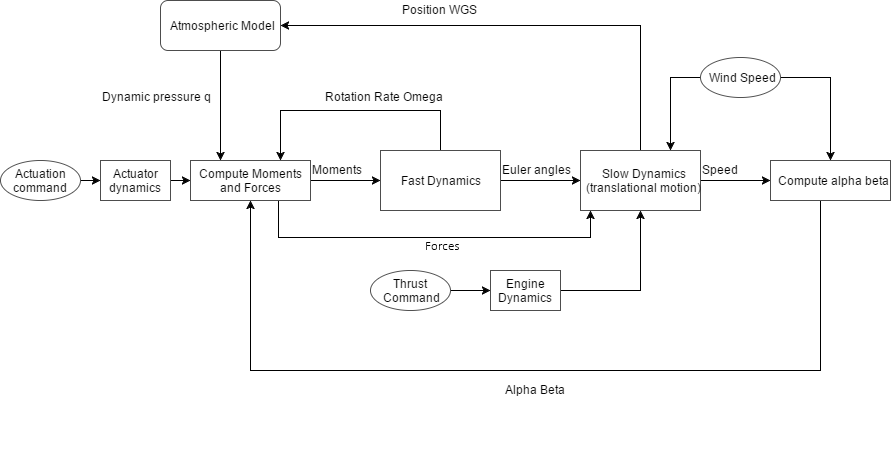
\includegraphics[width=0.75\textwidth]{../Figures/PlaneModel.png}
  \caption[Plane dynamics simulator diagram]{Plane dynamics simulator diagram}
  \label{fig:plane_model}
\end{figure*}
